% MiniCPM5-2B 双国产芯片推理吞吐优化技术报告
% 引擎：XeLaTeX（tectonic），ctex 中文支持
% 编译：xelatex -shell-escape main.tex（连续两遍；minted 需要 Pygments）
\documentclass[11pt,a4paper]{ctexart}
\usepackage[margin=2.5cm]{geometry}
\usepackage{microtype}
\usepackage{booktabs}
\usepackage{colortbl}
\usepackage{graphicx}
\usepackage{xcolor}
\usepackage{fancyhdr}
\usepackage{caption}
\usepackage{amsmath}
\usepackage{array}
\usepackage{tabularx}
\usepackage{subcaption}
\usepackage{float}
\usepackage{enumitem}
\usepackage{url}
\usepackage{setspace}
\setstretch{1.5}
\raggedbottom
\usepackage{listings}
\usepackage{minted}
\usepackage[most]{tcolorbox}
\usepackage{tikz}
\usetikzlibrary{arrows.meta,positioning,calc}
\definecolor{codeblue}{HTML}{0F4D92}
\definecolor{codeteal}{HTML}{0F766E}
\definecolor{codepurple}{HTML}{762A83}
\definecolor{codegray}{HTML}{6B7280}
\definecolor{codebg}{HTML}{F5F8FC}
\lstdefinestyle{reportcode}{
  basicstyle=\ttfamily\scriptsize,
  keywordstyle=\color{codeblue}\bfseries,
  stringstyle=\color{codeteal},
  commentstyle=\color{codegray}\itshape,
  numberstyle=\tiny\color{codegray},
  numbers=left,
  numbersep=6pt,
  stepnumber=1,
  frame=single,
  framerule=0.35pt,
  rulecolor=\color{lightgrey},
  backgroundcolor=\color{codebg},
  xleftmargin=1.6em,
  xrightmargin=0.5em,
  aboveskip=0.9em,
  belowskip=0.9em,
  breaklines=true,
  breakatwhitespace=false,
  columns=fullflexible,
  keepspaces=true,
  showstringspaces=false,
  tabsize=4,
  captionpos=b,
  emph={torch,triton,tl,mcblasGemmEx,flash_attn_varlen_func},
  emphstyle=\color{codepurple},
}
\lstset{style=reportcode}
\newtcolorbox{reportcode}[1]{
  colback=codebg,
  colframe=mainblue!35,
  colbacktitle=mainblue!10,
  coltitle=mainblue,
  title={#1},
  fonttitle=\small\heiti,
  arc=1.2pt,
  boxrule=0.35pt,
  left=0.8mm,
  right=0.8mm,
  top=0.5mm,
  bottom=0.5mm,
  before skip=0.9em,
  after skip=0.9em,
}
\newcommand{\PluginCode}{../pkg_build/XLANG2026/vllm-plugin-FL}
\newcommand{\GemsCode}{../pkg_build/XLANG2026/FlagGems}
\tikzset{
  flowbox/.style={draw=mainblue, fill=mainblue!5, rounded corners=2pt,
    align=center, font=\small, inner sep=5pt, minimum height=0.82cm},
  flowsmall/.style={flowbox, font=\scriptsize, inner sep=4pt},
  flowarrow/.style={-{Latex[length=2mm]}, thick, draw=mainblue},
  flownote/.style={font=\scriptsize\itshape\color{codegray}},
}
\graphicspath{{../submission/}}
\definecolor{mainblue}{HTML}{1F4E79}
\definecolor{accentred}{HTML}{A00000}
\definecolor{lightgrey}{HTML}{B8C0C8}
\pagestyle{fancy}
\fancyhf{}
\fancyhead[L]{\small MiniCPM5-2B 双国产芯片推理吞吐优化技术报告}
\fancyhead[R]{\small XLANG2026}
\fancyfoot[C]{\small \thepage}
\setlength{\headheight}{14pt}
\DeclareCaptionFont{hei}{\small\heiti}
\captionsetup{font=hei,labelfont={bf,color=mainblue},labelsep=quad,format=hang,justification=centering}
\captionsetup[sub]{font=hei,labelfont=bf,labelformat=parens,labelsep=quad,justification=centering,skip=4pt}
\newcolumntype{Y}{>{\raggedright\arraybackslash}X}
\setlist{itemsep=2pt,topsep=3pt}
\usepackage{hyperref}
\hypersetup{
  colorlinks=true,
  linkcolor=mainblue,
  urlcolor=mainblue,
  citecolor=mainblue,
  bookmarksnumbered=true,
  pdftitle={MiniCPM5-2B 双国产芯片推理吞吐优化技术报告},
  pdfauthor={XLANG2026 / 邓乾},
}
\title{\vspace{-1.2cm}\bfseries\LARGE MiniCPM5-2B 双国产芯片推理吞吐优化技术报告\\[4pt]
\large ——面向天数 BI-V150 与沐曦曦云 C500 的算子、内核与调度优化}
\author{赛道：FlagOS 开放计算全球大赛（赛季二）赛道二\\[2pt]
队伍：XLANG2026　队员：邓乾（GitHub：xy200303，单人组队）}
\date{2026 年 10 月 24 日}

\setlength{\emergencystretch}{2em}
\begin{document}
\maketitle
\thispagestyle{empty}

\begin{abstract}
\setlength{\parindent}{2em}
本报告面向国产芯片上的大模型推理吞吐优化任务，在官方指定的 FlagOS 栈（vllm-plugin-FL 分支 flagos-2026-s2、FlagGems 标签 v5.3.5）上，对 MiniCPM5-2B 在天数 BI-V150 与沐曦曦云 C500 两款芯片开展算子、内核与调度优化，保持 \texttt{vllm serve} 启动参数、模型与精度要求不变。

当前交付版本的 C500 复测中，4k 场景总吞吐为 12399.31 tok/s，是官网基线的 2.44 倍；16k 场景为 11046.19 tok/s，是基线的 1.57 倍。两项数据均来自同一实例、同一交付提交的官方四轮去首均值。天数 BI-V150 的官方开发与评测环境均为 32GB：两组 A20 的 4k 结果为 4087.91 和 4722.22 tok/s，A7 对照为 3855.31 和 3840.80 tok/s；16k 结果为 4520.19 和 4520.10 tok/s，A7 对照为 3568.31 和 3570.61 tok/s。A20 相对 A7 分别提升 6.0\%／22.9\%（4k）与 26.7\%／26.6\%（16k）。MATH-500 Level 3 中，C500 两次复测均为 98.1\%，BI-V150 为 96.19\% 和 98.1\%，均高于 95\% 的赛题要求。

主要优化包括：按输入形状选择 GEMM 与 attention 的实现或执行配置；用 1024-bin 质量直方图实现免排序 top-p 采样；针对 PV 矩阵乘的布局转换开销重写 paged decode attention，当前交付微基准由 stock 的 0.939 ms 降至 0.588 ms，有效带宽约 457 GB/s；减少 prefill 阶段的隐式同步与冗余内核发射。

\noindent\textbf{关键词：}国产芯片；推理吞吐；算子融合；paged decode attention；shape-aware dispatch；vLLM
\end{abstract}

\clearpage
\tableofcontents
\clearpage

\section{引言}
在硬件、框架和模型固定的条件下，推理吞吐主要受内核效率、访存布局、host 发射和同步开销影响。本报告以 MiniCPM5-2B\cite{minicpm} 为对象，在天数 BI-V150 与沐曦曦云 C500 上，基于官方指定的 FlagOS 软件栈（vllm-plugin-FL\cite{vfl} 与 FlagGems\cite{fg}）开展优化。

两种芯片在指令集、访存层次、运行时和算子库方面存在差异，通用 GPU 上的常用配置不一定适用。例如，Triton 默认的 \texttt{num\_warps=4, num\_stages=3} 在 BI-V150 的 decode attention 上并非合适选择。优化过程先用 profile 和微基准定位瓶颈，再修改内核或执行路径，最后通过官方 benchmark 和 MATH-500 评测端到端效果。后续章节分别介绍 C500 的采样链与 GEMM 路由、BI-V150 的 attention 接入与 decode 内核，以及正确性和复现方法。

\subsection{任务定义}
本赛题要求在不改变模型、不降低精度的前提下，提升 MiniCPM5-2B 在两指定国产芯片上的推理总吞吐（total tokens/s）。优化必须落在框架与算子内部，且需具备实际开发量：KV Cache 与动态批处理、算子融合、内核重写、自研量化策略等均在允许范围内；直接 merge 上游分支、修改 benchmark 脚本、或在缺乏算子优化的情况下切换算子均被禁止。

\subsection{评测口径}
\begin{table}[!htbp]
\centering
\caption{官方性能评测场景与约束}
\begin{tabularx}{\linewidth}{@{}p{2.6cm}Y@{}}
\toprule
项目 & 内容 \\
\midrule
性能指标 & total tokens/s（总吞吐，取 4k 与 16k 两场景平均）\\
4k 场景 & [4096, 1024, 64, 256]（输入长、输出长、并发、请求数）\\
16k 场景 & [16384, 1024, 64, 128]\\
精度要求 & MATH-500 Level 3，基线 0.962，要求 $\geq 0.95$\\
TTFT 要求 & 不得超过基线的 $+1\%$\\
启动参数 & \texttt{vllm serve} 参数必须与基线完全一致\\
\bottomrule
\end{tabularx}
\end{table}

性能数字均由官方 \texttt{vllm bench serve} 产生。当前 C500 复测与历史 opt 系列均采用同一服务连续四轮、去首轮后三轮均值；连续运行不保证每轮冷缓存，prefix cache 命中情况逐次查日志。精度数字来自 evalscope 官方原命令的 MATH-500 Level 3 子集（105 题）。

\section{总体成绩}
当前 C500 数据来自同一健康实例、同一交付提交的完整复测，并同时保留官网基线和本机原生基线。天数 BI-V150 的官方开发与评测环境均为 32GB；相对收益采用同日交错 A/B，避免跨时段漂移的影响。

\subsection{交付版本与启动验证}
交付代码为插件与算子两个独立仓库中的固定提交，均保留完整 Git 历史，可用 \texttt{git log}、\texttt{git show} 和 \texttt{git diff} 查看改动。

\begin{table}[!htbp]
\centering
\caption{代码版本与记录入口}
\begin{tabularx}{\linewidth}{@{}p{2.0cm}p{4.0cm}Y@{}}
\toprule
组件 & 仓库 / 分支 & 固定提交与内容 \\
\midrule
插件 & \path{xy200303/vllm-plugin-FL}\newline \path{integration/vllm-plugin-fl} & \texttt{0207b7e1}；C500 opt1–opt11、BI-V150 A1–A7、A20 框架 hook \\
算子 & \path{xy200303/FlagGems}\newline \path{integration/flaggems} & \texttt{aff68555}；采样、GEMM、paged decode attention 与测试 \\
文档 & \path{xy200303/minicpm-flagserve}\newline \texttt{main} & 报告、实验台账、复现脚本；不承担运行时代码 \\
\bottomrule
\end{tabularx}
\end{table}

2026-10-25 在 C500（64GB 显存、128GB CPU 内存）上，从上述提交部署并显式固定源码路径。交付版启动耗时 293 秒，日志包含 \texttt{mcblas\_mm} 注册、采样融合启用和 lm\_head nn 路由；原生基线启动耗时 161 秒。两者均完成官方四轮 benchmark，当前交付版另完成两次 MATH-500 评测。

\begin{table}[!htbp]
\centering\small
\caption{官网基线、原生栈复测与当前交付的总吞吐（tok/s）}
\begin{tabularx}{\linewidth}{@{}l l r r r Y@{}}
\toprule
平台 & 场景 & 官网基线 & 原生栈复测 & 当前交付 & 相对官网 \\
\midrule
沐曦 C500 & 4k & 5089.645 & 4210.20 & 12399.31 & 2.44$\times$\\
沐曦 C500 & 16k & 7029.675 & 5867.59 & 11046.19 & 1.57$\times$\\
天数 BI-V150 & 4k & 2028.01 & 1902.15 & 4087.91–4722.22 & 2.02$\times$–2.33$\times$\\
天数 BI-V150 & 16k & 915.15 & 861.98 & 4520.10–4520.19 & 4.94$\times$\\
\bottomrule
\end{tabularx}
\end{table}

原生栈复测均使用未修改的官方栈、官方启动命令和四轮去首均值：C500 测于 2026-10-25，BI-V150 测于 2026-10-10（32GB 官方实例）。BI 原生数据及逐轮值见 \path{docs/baselines/iluvatar-biv150/a1-iluvatar-vendor-fa.md}；因实例和日期不同，只用于区分官网数字、原生复现与最终交付，不替代文中的同日 A/B 对照。

注意，total tok/s 同时计入输入与输出，且 4k／16k 的请求数分别为 256／128，不能用该指标直接比较单请求速度。以 BI-V150 第一组为例，两场景总 token 分别为 1.31M／2.23M，因此 16k 总吞吐可接近 4k；同组 decode 输出吞吐则由 817.58 降至 265.89 tok/s，TTFT 由 4.33 s 增至 111.64 s，长上下文成本体现在这些分项指标中。

C500 的本机原生基线为 4k 4210.20、16k 5867.59 tok/s，当前交付相对其分别为 2.95$\times$ 和 1.88$\times$。C500 两次 MATH-500 Level 3 均为 98.1\%，BI-V150 为 96.19\% 和 98.1\%，每次均 105/105 请求成功。C500 的 4k TTFT 为 1719.18 ms（官网基线 3199.435 ms），16k TTFT 为 18141.47 ms（官网基线 27197.135 ms）；BI-V150 的 4k TTFT 为 4139.85–4327.86 ms（官网基线 11573.53 ms），16k TTFT 为 111.64–111.67 s（官网基线 599262.03 ms；A7 对照为 136.86–137.00 s）。按官网基线判断，两平台各场景均满足 TTFT 不超过 baseline +1\% 的约束。

\subsection{性能与约束对照}
图~\ref{fig:compliance} 汇总吞吐、精度和 TTFT 相对裕度。吞吐与 TTFT 取相对基线的改善百分比，精度取相对 0.95 门槛的提升幅度。C500 四项数值为 +143.6\%／+57.1\%／+3.3\%／+33.3\%，BI-V150 为 +101.6\%／+393.9\%／+1.3\%／+81.4\%。

\begin{figure}[!htbp]
\centering
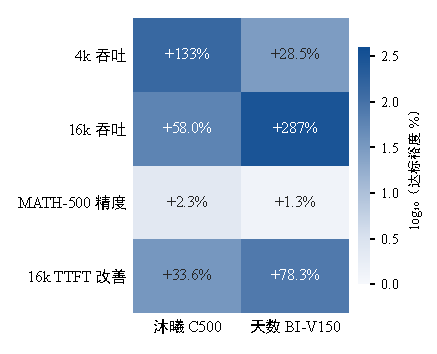
\includegraphics[width=0.495\linewidth]{fig15_compliance.pdf}
\caption{四项硬约束的达标裕度（相对各自门槛的百分比，颜色取 $\log_{10}$）\label{fig:compliance}}
\end{figure}

\begin{figure}[!htbp]
\centering
\begin{minipage}[b]{0.495\linewidth}
  \centering
  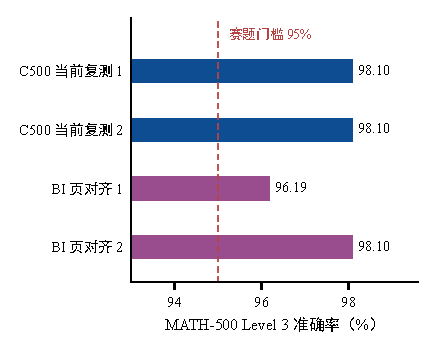
\includegraphics[width=\linewidth]{fig8_accuracy.pdf}
  \subcaption{MATH-500 Level 3 精度与合格线}
\end{minipage}\hfill
\begin{minipage}[b]{0.495\linewidth}
  \centering
  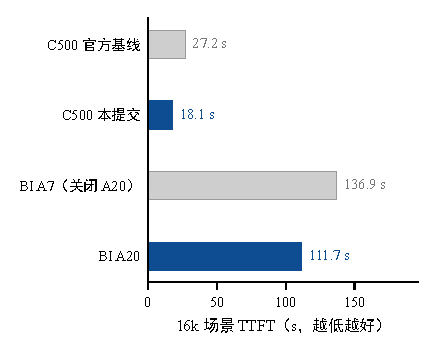
\includegraphics[width=\linewidth]{fig9_ttft.pdf}
  \subcaption{16k 场景 TTFT（越低越好）}
\end{minipage}
\caption{精度与延迟两项约束的对照：四个平台／场景组合均达标}
\end{figure}

\begin{figure}[!htbp]
\centering
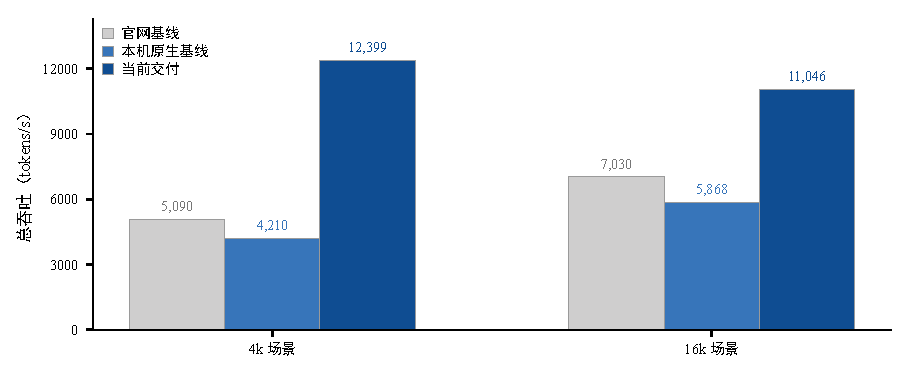
\includegraphics[width=\linewidth]{fig1_c500_throughput.pdf}
\caption{沐曦 C500：官网基线、本机原生基线与当前交付的四轮去首均值对比}
\end{figure}

\begin{figure}[!htbp]
\centering
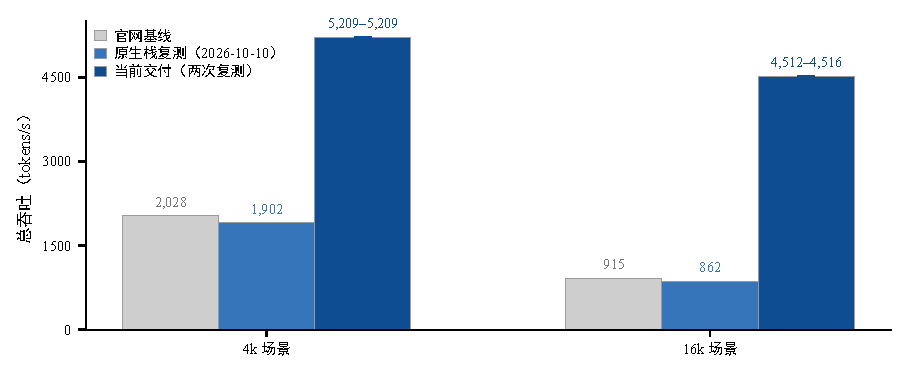
\includegraphics[width=\linewidth]{fig20_bi_three_way.pdf}
\caption{天数 BI-V150：官网基线、历史原生栈复测与当前交付对比；误差线保留两次交付复测范围，原生复测与交付复测不视为同日 A/B}
\end{figure}

\subsection{实验环境}
表~\ref{tab:environment} 列出最终复测环境。硬件容量、驱动与运行时来自实例管理接口，依赖版本来自 Python 包信息；BI-V150 的 Triton 版本采用运行时 \texttt{triton.\_\_version\_\_} 读数。两平台使用同一组交付提交，避免把代码差异混入平台对比。

\begin{table}[!htbp]
\centering\small
\caption{双平台最终复测的软硬件环境\label{tab:environment}}
\begin{tabularx}{\linewidth}{@{}p{2.6cm}YY@{}}
\toprule
项目 & 天数 BI-V150 & 沐曦曦云 C500 \\
\midrule
GPU / 显存 & BI-V150 / 32GB & C500（104 SM）/ 64GB \\
CPU & Intel Xeon Gold 6330 @ 2.00GHz & Intel Core i7-8550U \\
CPU 内存 / Swap & 503GiB / 8GiB & 128GiB / 无 \\
实例与镜像 & FlagOS 线上实验室官方环境 & 模力方舟，FlagOS 2.1 \\
PyTorch & 2.10.0+corex.4.5.0 & 2.8.0+metax3.7.0.7 \\
vLLM & 0.24.0 & 0.24.0 \\
Triton & 3.6.0 & 3.0.0+metax3.7.0.7 \\
芯片软件栈 & IX-ML 4.4.0；驱动 4.5.0 & MACA 3.7.0.38；驱动 3.8.30 \\
evalscope & 1.11.1 & 1.11.1 \\
插件 / FlagGems & 0207b7e1 / aff68555 & 0207b7e1 / aff68555 \\
最终复测日期 & 2026-10-26 至 2026-10-27 & 2026-10-25 \\
\bottomrule
\end{tabularx}
\end{table}

C500 的 CPU 内存是本队实例的实测复现条件，不是官网公布的评测规格；CPU 型号来自同镜像开发实例记录，最终复测 manifest 未重复采集该字段。64GB CPU 内存实例上原生镜像也曾发生启动期 OOM，因此复现说明单独保留这一现象与内存建议。BI-V150 的 32GB 指 GPU 显存，不能与 CPU 内存混淆。

\subsection{关键优化点}
本提交的技术路线由以下三部分组成，详细实现和实验分别见第 4、5 章。

\textbf{（1）面向芯片与输入形状的执行路径选择。} 不假定同一 GEMM 或 attention 配置在所有形状上最优，而是在保留原实现的前提下，按 M、KV 页尺寸和 prefill／decode 类型选择 vendor 库或 Triton 内核。C500 侧重 lm\_head 与 prefill GEMM 的布局、库调用和 host 元数据路径；BI-V150 侧重 warp 级发射配置与 attention 实现。路由之外还包含权重复本、布局转换、同步消除和页对齐访问等代码改动。

\textbf{（2）免排序 top-p 采样与温度折叠。} 将 bf16 logits 读取、top-p 阈值估计、掩码与 Gumbel-Max 合并，避免对 130560 词表进行完整排序。阈值由 1024-bin 质量直方图定位并保守取 bin 下沿；温度通过 $\arg\max(x/T+g)=\arg\max(x+Tg)$ 折叠进采样分数。该路径直接作用于每步解码末尾的采样热点。

\textbf{（3）减少 PV 布局转换的 paged decode attention。} 针对 BI-V150 上 PV 矩阵乘的累加器到操作数布局转换，将并行单元组织为 warp 内的（序列、KV 头、分段）计算，配合单 warp 发射、base-2 在线 softmax 和分段归并。段边界与 KV 页对齐后，页号在段内保持标量，省去逐 token 除模和向量页 gather；段长由设备端 \texttt{seq\_lens} 计算，分段缓存在图捕获前分配，以兼容 FULL\_DECODE\_ONLY。

\section{优化流程}
两种芯片采用相同的分析与验证流程，测试脚本、profile、日志和 benchmark CSV 按实验编号保存。

\begin{figure}[!htbp]
\centering
\begin{tikzpicture}[font=\small]
  \node[flowbox, minimum width=3.1cm] (serve) at (0,0) {\texttt{vllm serve}\\官方启动参数};
  \node[flowbox, minimum width=3.1cm] (dispatch) at (4.0,0) {vllm-plugin-FL\\dispatch / hook};
  \node[flowbox, minimum width=3.1cm] (kernels) at (8.0,0) {FlagGems / vendor\\Triton · mcBLAS · ixAttnBkd};
  \node[flowbox, minimum width=3.1cm] (gpu) at (12.0,0) {BI-V150 / C500\\GPU 执行};
  \node[flowsmall, minimum width=3.1cm] (fallback) at (4.0,-1.8) {stock 路径\\按实现回退};
  \node[flowsmall, minimum width=3.1cm] (evidence) at (8.0,-1.8) {profile · A/B · 精度\\CSV · 日志 · 单测};
  \draw[flowarrow] (serve) -- (dispatch);
  \draw[flowarrow] (dispatch) -- (kernels);
  \draw[flowarrow] (kernels) -- (gpu);
  \draw[flowarrow, dashed] (dispatch) -- (fallback);
  \draw[flowarrow, dashed] (dispatch) -- (evidence);
  \node[flownote] at (6.0,-2.65) {保留 stock 回退路径与原始测试记录};
\end{tikzpicture}
\caption{插件、算子实现与测试记录之间的关系}
\end{figure}

算子本体位于 FlagGems，框架接入位于 vllm-plugin-FL。性能测试使用官方 benchmark，精度测试使用 evalscope，内核测试与实现文件按附录索引对应。A20、vendor prefill 和不支持的采样特征保留回退路径；mcBLAS 返回码采用断言检查，不属于异常自动回退。

（1）Profile 定位：结合 serve 时序日志（PagedAttention 式分页 KV 管理见文献\cite{vllm}）、设备计时与 host 打点，区分 GPU 内核、host 发射和隐式同步开销；（2）独立测试：新内核先检查目标形状的数值结果，再接入 serve；（3）Shape-aware dispatch：按输入形状选择等价实现或执行配置；（4）端到端测试：保持官方 serve 参数，检查吞吐、TTFT 和 MATH-500 精度。

A6 双 gather、A7 发射配置要求逐位一致；采样融合与 GEMM 路由检查分布和数值误差，并复测 MATH-500。不满足精度要求的改动不进入交付分支。

\section{沐曦 C500：采样链、GEMM 路由与 host 同步消除}
\subsection{瓶颈画像}
初始 profile 显示，C500 的主要开销集中在采样、GEMM 和 attention。采样尾部采用 eager PyTorch 实现，包括 bf16$\rightarrow$fp32 cast、温度缩放、130560 词表排序和 gumbel-argmax；部分 GEMM 存在布局与路由失配；prefill 的隐式 DtoH 同步则造成 GPU 空闲。

图~\ref{fig:hotpath} 将 opt1 前后同一基准（641 步）两次 profile 的 GPU 内核时间按算子族聚合（源：\path{docs/baselines/metax-c500/profile_baseline.txt} 与 \texttt{profile\_post\_opt1.txt}）。采样族由 14.61 s 降至 1.24 s，占内核时间的比例由 38.8\% 降至 5.1\%；GEMM 与 attention 的绝对时间分别为 13.82$\rightarrow$13.81 s、7.19$\rightarrow$7.22 s。该图不代表 opt11 最终 profile，后续优化分别针对 GEMM 路由、attention 和 prefill 同步展开。

\begin{figure}[!htbp]
\centering
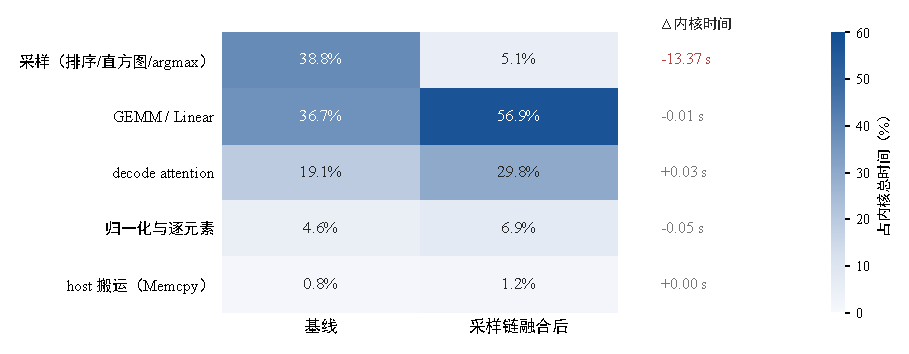
\includegraphics[width=\linewidth]{fig14_op_hotpath.pdf}
\caption{C500 opt1 前后热路径的算子族构成：按内核时间占比（右列为绝对时间变化）\label{fig:hotpath}}
\end{figure}

\subsection{免排序的采样链（opt1／opt3／opt7／opt11）}
自研 Triton 内核（\texttt{FlagGems/fused/sampler\_fused.py}、\texttt{top\_p\_sample.py}）做三件事：其一，直接以 bf16 读取 lm\_head 输出，把温度折叠进 Gumbel-Max\cite{gumbel}（$\arg\max(x/T+g)$ 与 $\arg\max(x+T\cdot g)$ 等价，$T<10^{-5}$ 时退化为 $\arg\max$）；其二，top-p 用质量直方图 zoom，单轮 1024-bin 直方图定位阈值 $\tau$ 所在 bin 并取其下沿，在忽略 $\exp(-60)$ 截断尾质量的近似下，保留集质量不小于 $p\cdot Z$；其三，官方 B=64 形状采用词表维 split-parallel（32 splits $\times$ BLOCK 4096）。2026-10-25 在当前交付代码上复测，B=64、词表 130560 时，同语义 PyTorch top-p 对照为 4.086 ms，\texttt{fused\_top\_p\_sample} 为 0.381 ms，约 10.7$\times$。

\begin{figure}[!htbp]
\centering
\begin{tikzpicture}[font=\scriptsize]
  \draw[fill=mainblue!8, draw=mainblue] (0,0) rectangle (10,0.62);
  \foreach \x in {1,...,9} \draw[mainblue!45] (\x,0) -- (\x,0.62);
  \draw[fill=mainblue!25] (6.4,0) rectangle (10,0.62);
  \draw[accentred, thick] (6.4,-0.25) -- (6.4,0.94);
  \node[accentred, above] at (6.4,0.94) {$\tau$：跨界 bin 的下沿};
  \node[codegray, below] at (2.7,-0.10) {1024-bin 质量直方图};
  \node[mainblue, below] at (8.2,-0.10) {保留集质量 $\geq pZ$（截断近似）};
  \node[flowsmall] (stats) at (0,-1.55) {bf16 直读\\$x/T$ 与 $Z$};
  \node[flowsmall] (hist) at (3.3,-1.55) {反向 cumsum\\定位跨界 bin};
  \node[flowsmall] (tau) at (6.6,-1.55) {保守取下沿 $\tau$\\不过度裁剪};
  \node[flowsmall] (sample) at (9.9,-1.55) {mask + Gumbel-Max\\一趟产出 token};
  \draw[flowarrow] (stats) -- (hist);
  \draw[flowarrow] (hist) -- (tau);
  \draw[flowarrow] (tau) -- (sample);
\end{tikzpicture}
\caption{免排序 top-p 采样链示意图（流程与阈值规则为代码语义，非另造的分布数据）\label{fig:topp}}
\end{figure}

图~\ref{fig:topp} 中的阈值取所在 bin 的下沿；忽略 $\exp(-60)$ 截断尾质量时，保留集质量不小于 $pZ$，因此该下界带截断近似限定。采样分数写成 $x+Tg$，与先算 $x/T$ 再加 $g$ 的 argmax 等价。对应实现如下。

\begin{reportcode}{\texttt{top\_p\_sample.py:180--198}：反向 cumsum 定位阈值并保守取下沿}
\inputminted[linenos,fontsize=\scriptsize,breaklines,tabsize=4,firstline=180,lastline=198]{python}{\GemsCode/src/flag_gems/fused/top_p_sample.py}
\end{reportcode}

\begin{reportcode}{\texttt{top\_p\_sample.py:241--249}：温度折叠的 Gumbel-Max 与 top-p mask}
\inputminted[linenos,fontsize=\scriptsize,breaklines,tabsize=4,firstline=241,lastline=249]{python}{\GemsCode/src/flag_gems/fused/top_p_sample.py}
\end{reportcode}

正确性方面，greedy 与 \texttt{torch.argmax} 完全一致；top-p 样本全部落在核集内（含直方图粒度 slack），与原实现的 TV 距离处于纯采样噪声区间。

\begin{figure}[!htbp]
\centering
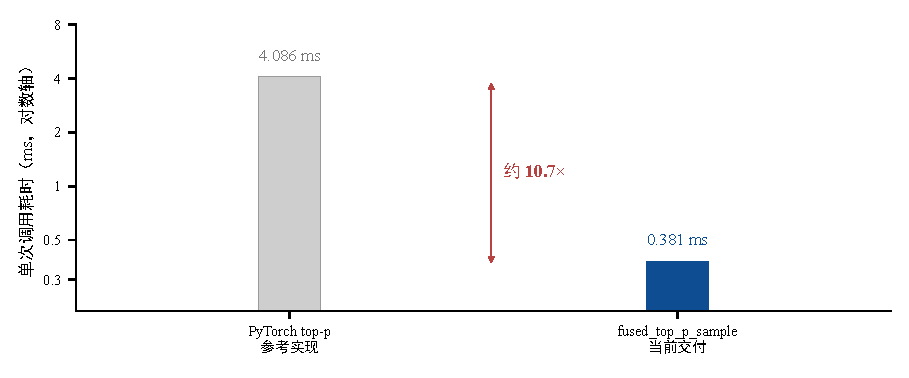
\includegraphics[width=\linewidth]{fig2_sampler.pdf}
\caption{当前交付 top-p 采样与同语义 PyTorch 对照（B=64，30 次中位数，对数坐标）}
\end{figure}

\subsection{GEMM 布局与路由（opt2／opt4／opt6／opt8／opt11）}
MACA Triton \texttt{mm\_kernel} 的高性能流水主要适配 nn 布局。在 prefill 大 M 的 126 组配置扫描中，其耗时为 vendor mcBLAS 的 1.35–1.67 倍；四种 prefill 形状的 vendor 计算吞吐约为 152–197 TFLOPS。FlagGems 接管 \texttt{aten::mm} 后，原路由无法直接调用 vendor GEMM。为此，prefill 大 M 通过 ctypes 调用 libmcblas 的 \texttt{mcblasGemmEx}（cuBLAS 兼容 ABI），并注册为 custom op 以适配 compiled 区域。默认配置为双布局：小 M（默认阈值 192）或缺少 nn 副本时回退 \texttt{F.linear}，大 M 按路由使用 Triton nn 或 mcBLAS；仅保留 nn\_db 副本的单布局配置可选，但不是默认。另修复 \texttt{vocab\_parallel\_embedding} 在 import 时绑定原版 \texttt{dispatch\_unquantized\_gemm} 导致 lm\_head 未进入优化路由的问题。2026-10-25 复测该形状时，FlagGems Triton 为 667 $\mu$s，直接 mcBLAS 为 430 $\mu$s（1.55$\times$）；同次原生 \texttt{torch.mm} 为 385 $\mu$s，说明 mcBLAS 的收益是相对于 FlagGems 路径，而不是超过所有 vendor 实现。

只有已经生成 nn 副本且形状满足条件的线性层才进入新路径。lm\_head 通过独立的 \texttt{\_fl\_always\_nn} 标志使用 nn 副本，避免被通用 N 上限排除。

\begin{reportcode}{\texttt{linear\_nn\_repack.py:112--136}：按形状在 vendor、Triton 与 stock 之间路由}
\inputminted[linenos,fontsize=\scriptsize,breaklines,tabsize=4,firstline=112,lastline=136]{python}{\PluginCode/vllm_fl/dispatch/backends/vendor/metax/patches/linear_nn_repack.py}
\end{reportcode}

ctypes 绑定把行主序的 $C=A B$ 转写成列主序的 $C^T=B^T A^T$，因此不需要改变模型的数学结果；\texttt{register\_fake} 让编译器在 fake tensor 阶段仍能推导输出形状。

\begin{reportcode}{\texttt{mcblas\_mm.py:85--103}：直接调用 mcBLAS，保持原 GEMM 语义}
\inputminted[linenos,fontsize=\scriptsize,breaklines,tabsize=4,firstline=85,lastline=103]{python}{\PluginCode/vllm_fl/dispatch/backends/vendor/metax/patches/mcblas_mm.py}
\end{reportcode}

\subsection{消除 prefill 每层 DtoH 同步（opt10）}
prefill trace 中，相邻 GPU 内核间隔大于 20 $\mu$s 的 gap 占 18.1\%；元凶之一是 vendor flash\_attn 每层每步执行 \path{prefill_seq_lens.tolist()}（DtoH 强同步，42 层各一次）。改为纯 GPU cumsum 并缓存到当步 \texttt{attn\_metadata}，42 层只算一次：4k 提升 10.9\%、16k 提升 9.9\%，16k TTFT 由 20.8 s 降至 18.0 s。

\begin{reportcode}{\texttt{flash\_attn.py:797--811}：把每层一次的 DtoH + cumsum 改成当步缓存}
\inputminted[linenos,fontsize=\scriptsize,breaklines,tabsize=4,firstline=797,lastline=811]{python}{\PluginCode/vllm_fl/dispatch/backends/vendor/metax/impl/attention/flash_attn.py}
\end{reportcode}

这段代码只改变 metadata 的生产方式，不改变请求组成、调度顺序或 \texttt{vllm serve} 参数；缓存对象仍然属于当前 \texttt{attn\_metadata}，不会跨请求复用旧长度。

\begin{figure}[!htbp]
\centering
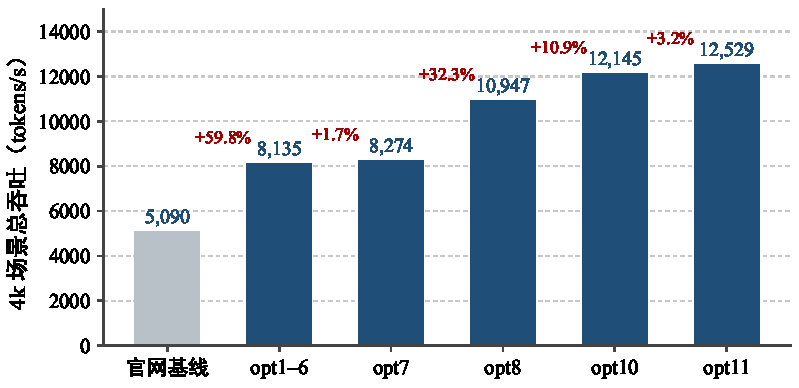
\includegraphics[width=\linewidth]{fig3_c500_ladder.pdf}
\caption{C500 4k 场景历史版本优化阶梯（含跨实例记录，非严格同机累计 A/B）}
\end{figure}

\section{天数 BI-V150：vendor 接入、发射配置与自研 decode 内核}
\subsection{瓶颈画像}
BI-V150 的瓶颈随优化阶段发生变化。初始 16k prefill 中，vLLM 通用 Triton \path{kernel_unified_attention} 占 GPU 忙时的 91.8\%，每层每 2048-token chunk 耗时 36.8 ms；此时 GPU busy 为 99.1\%，主要开销来自 attention 内核本身。iluvatar 后端缺少 flash\_attn 包，是这条慢路径的直接原因。

接入 vendor attention 后，混合步的主要开销转移到 host 侧。A1.5 的 16k 混合步 wall 约为 677 ms，GPU busy 为 41.3\%，按此折算 GPU 工作约 280 ms、host 等待约 397 ms。builder 中两处 GPU 张量高级索引触发阻塞式 HtoD 和全流同步，每次中位耗时 78.6 ms。A3 将 metadata 构建移到 CPU 侧并减少重复发射后，wall 降至 353 ms，GPU busy 提升到 76.3\%。decode 侧则另有发射配置与 PV 布局转换开销，分别在后续两节展开。

\begin{figure}[!htbp]
\centering
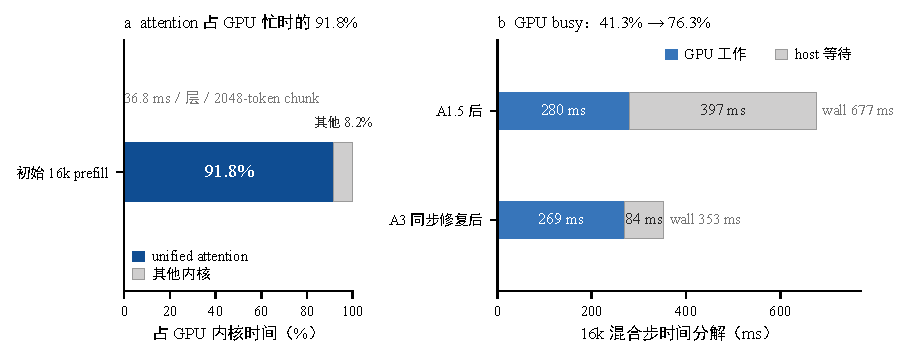
\includegraphics[width=\linewidth]{fig19_biv150_bottleneck.pdf}
\caption{BI-V150 的 prefill 内核构成与接入 vendor 后的混合步时间分解\label{fig:biv150_bottleneck}}
\end{figure}

\subsection{prefill attention 与 host 路径（A1／A3／A6）}
针对上述瓶颈，接入 vendor ixAttnBkd 内核，并确认其 causal 语义为 bottom-right（cmt=2），与 vLLM 的 chunk prefill 对齐。内核级实测在所有 kv 长度上均快 12–20 倍。配套地，builder 一次性完成每步 decode/prefill 划分，避免每层两次 D2H；KV 用自研 Triton \texttt{\_dual\_gather\_kernel} 一次完成 K+V 分页收集（bit-exact，GPU 106$\rightarrow$62 $\mu$s、host 68$\rightarrow$37 $\mu$s），varlen 分支用 out= 直写消除 copy-out，每请求发射数由 4 降为 2。

\begin{reportcode}{\texttt{vendor\_flash\_attn.py:46--57}：同一 Triton program 收集一页 K 与 V}
\inputminted[linenos,fontsize=\scriptsize,breaklines,tabsize=4,firstline=46,lastline=57]{python}{\PluginCode/vllm_fl/dispatch/backends/vendor/iluvatar/impl/vendor_flash_attn.py}
\end{reportcode}

其中 \texttt{E=bs*hkv*d} 是一页 K 的元素数，V 的源地址位于 K 之后的连续区域。内核利用这一布局在同一 program 中收集 K 和 V，数值测试与两次 \texttt{index\_select} 逐位一致。

\subsection{decode unified-attention 发射配置重构（A7）}
stock Triton 默认 \texttt{num\_warps=4, num\_stages=3}。扫描结果表明，该配置在 BI-V150 上并不合适，软件流水线在各 warp 档上均未带来收益。对 3D 主内核与 reduce\_segments 全链路扫描后，将 3D flash-decoding 路径固定为 w1 s1，保持 TILE=16、SEG=16，2D 路径不变；输出与 stock 逐位一致。

\begin{reportcode}{\texttt{decode\_attn\_pin.py:35--47}：只包住 3D 内核的发射配置，2D 路径不变}
\inputminted[linenos,fontsize=\scriptsize,breaklines,tabsize=4,firstline=35,lastline=47]{python}{\PluginCode/vllm_fl/dispatch/backends/vendor/iluvatar/impl/decode_attn_pin.py}
\end{reportcode}

\begin{figure}[!htbp]
\centering
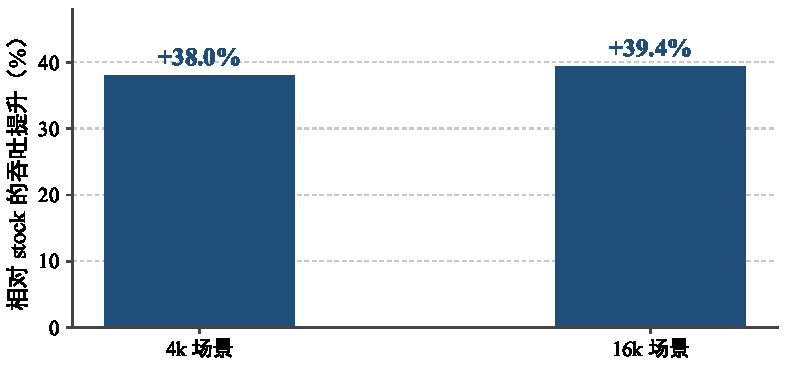
\includegraphics[width=\linewidth]{fig7_a7_config.pdf}
\caption{A7 发射配置重构带来的端到端吞吐提升}
\end{figure}

\subsection{自研 paged decode attention 内核（A20）}
A7 之后，decode attention 仍占整步的主要时间。在同一 harness 下逐段测量 stock kernel（B=64／kv=4096／16q-2kv／d=128／block=16／bf16）：loads+QK 的有效带宽为 509 GB/s，PV 的 \texttt{tl.dot} 耗时 0.36 ms。PV 需要将 p 从 MMA 累加器布局转换为 A 操作数布局，每个 KV block 都产生共享内存往返，因此本阶段的主要开销是布局转换。

据此重写内核（算子位于 \texttt{FlagGems/fused/paged\_decode\_attention.py}，插件侧为薄封装与派发）：一个 CTA＝1 warp＝一个（seq, kv\_head, 段），使布局转换留在 warp 内；BLOCK\_N=16，p tile 不超过一个 MMA 形状；base-2 在线 softmax，scale 预折 $\log_2(e)$ 走 MUFU；主循环不加 mask，仅 ragged 尾部单独一个带 mask 的 block；段数固定、段长由 device 端 seq\_lens 现算（CUDA-graph 安全），段缓存 slab 在 \texttt{apply()} 即捕获前一次性预分配；段边界按整页对齐，进一步消去逐 token 除模与向量页 gather。混合步中的 decode 行也通过 \texttt{try\_fast\_decode} 进入同一内核。

\begin{figure}[!htbp]
\centering
\begin{tikzpicture}[font=\scriptsize]
  \node[flowsmall] (input) at (0,0) {q / K / V\\block\_table + seq\_lens};
  \node[flowsmall] (split) at (4.0,0) {固定 NSEG=32\\按整页分段};
  \node[flowsmall] (warp) at (8.0,0) {每段 1 warp\\base-2 在线 softmax};
  \node[flowsmall] (combine) at (12.0,0) {combine 归并\\输出 attention};
  \draw[flowarrow] (input) -- (split);
  \draw[flowarrow] (split) -- (warp);
  \draw[flowarrow] (warp) -- (combine);
  \node[flownote] at (6.0,-1.15) {主循环无 mask；仅 ragged 尾块 mask；段长 device 端计算，slab 在图捕获前预分配};
\end{tikzpicture}
\caption{A20 paged decode attention 的分段执行与归并流程}
\end{figure}

下面的主循环展示了三个直接针对瓶颈的选择：页边界对齐后 \texttt{page} 只需标量加载；\texttt{exp2} 代替 \texttt{exp}；每段只写自己的 \texttt{SEG\_ACC/SEG\_MAX/SEG\_SUM}，最后由 combine 按 $\exp2(m_i-m)$ 加权归并。

\begin{reportcode}{\texttt{paged\_decode\_attention.py:169--193}：页对齐主循环与 base-2 在线 softmax}
\inputminted[linenos,fontsize=\scriptsize,breaklines,tabsize=4,firstline=169,lastline=193]{python}{\GemsCode/src/flag_gems/fused/paged_decode_attention.py}
\end{reportcode}

\begin{reportcode}{\texttt{paged\_decode\_attention.py:207--223}：分段结果的在线归并}
\inputminted[linenos,fontsize=\scriptsize,breaklines,tabsize=4,firstline=207,lastline=223]{python}{\GemsCode/src/flag_gems/fused/paged_decode_attention.py}
\end{reportcode}

\begin{figure}[!htbp]
\centering
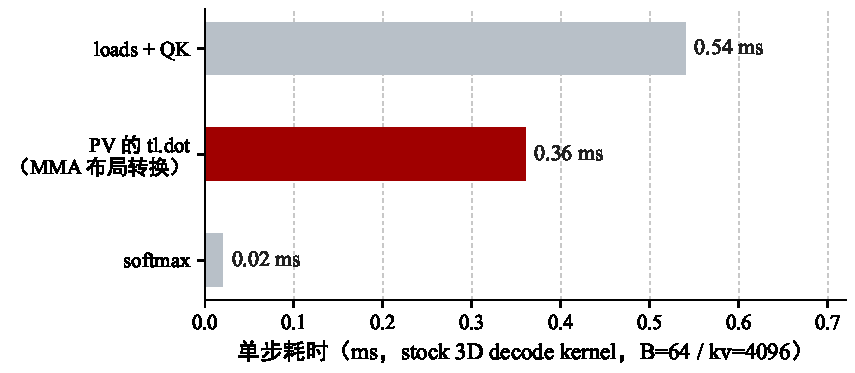
\includegraphics[width=\linewidth]{fig6_decode_breakdown.pdf}
\caption{stock 3D decode 内核的耗时分解：瓶颈在 PV 的 MMA 布局转换}
\end{figure}

当前交付的页对齐微基准中，stock 为 0.939 ms/层、286 GB/s，A20 为 0.588 ms/层、457 GB/s，加速比 1.60$\times$；等长与 ragged 的最大误差分别为 $3.05\times10^{-5}$ 和 $6.10\times10^{-5}$。两组官方 A/B 的 4k 结果为：A7 3855.31→A20 4087.91（+6.0\%），A7 3840.80→A20 4722.22（+22.9\%）；16k 结果为：A7 3568.31→A20 4520.19（+26.7\%），A7 3570.61→A20 4520.10（+26.6\%）。两组 16k TTFT 分别为 111.64 s 和 111.67 s，较 A7 降低 18.5\% 和 18.4\%。当前交付两次 MATH-500 Level 3 为 96.19\% 和 98.1\%。

\begin{figure}[!htbp]
\centering
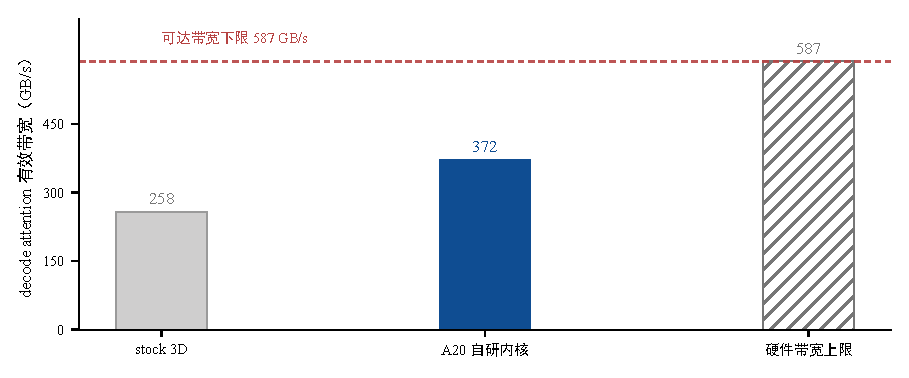
\includegraphics[width=\linewidth]{fig4_decode_bw.pdf}
\caption{stock 与页对齐版本的 decode attention 有效带宽对比（kv=4096，B=64）}
\end{figure}

\begin{figure}[!htbp]
\centering
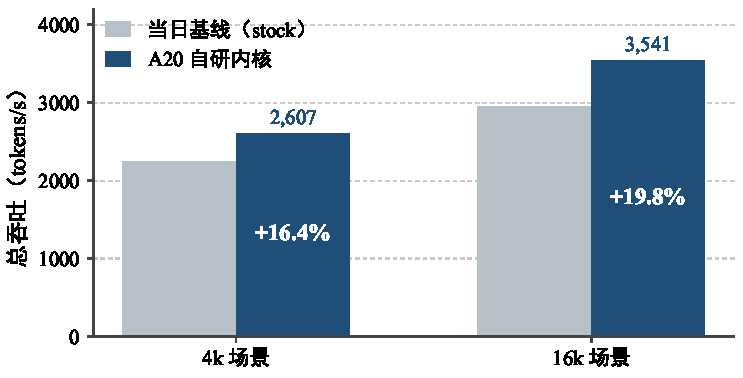
\includegraphics[width=\linewidth]{fig5_iluvatar_ab.pdf}
\caption{BI-V150 两组官方 A/B：A7 栈关闭 A20 与当前 A20 的对比}
\end{figure}

\subsection{批量一致性与路径检查}
每个（seq, kv\_head, segment）只依赖自身的 q、KV 页和 seq\_lens，段长仅由序列长度决定。交付中的 \path{tests/test_paged_decode_attention.py} 包含 8 个 fp32 参考对照用例和一个批量不变性用例，在 BI-V150 上实测 \textbf{9 passed}。批量测试覆盖单条、两条、半批、全批和逆序全批，并重复执行同一批组成。混合步的 decode 切片每 4000 次调用记录 used/skipped；当前日志为 used=132000、skipped=0。

\begin{reportcode}{\texttt{decode\_attn\_fast.py:186--205}：混合步 decode 切片的资格检查、计数与异常回退}
\inputminted[linenos,fontsize=\scriptsize,breaklines,tabsize=4,firstline=186,lastline=205]{python}{\PluginCode/vllm_fl/dispatch/backends/vendor/iluvatar/impl/decode_attn_fast.py}
\end{reportcode}

满足形状与特征条件时进入新内核；遇到不支持的特征或异常则回到原实现。used 在内核执行前递增，表示通过资格检查并尝试 fast path；本次同时检查了 fallback 日志，未出现 decode fast-path 异常回退。

\subsection{跨平台结果对照}
图~\ref{fig:incremental} 对比两种芯片的历史收益构成。C500 的 opt1–opt6 包含跨实例版本记录，展示开发过程而非严格同机累计 A/B；BI-V150 的 A6、A7、A20 使用各自的当日对照，三组数据不作累计。

\begin{figure}[!htbp]
\centering
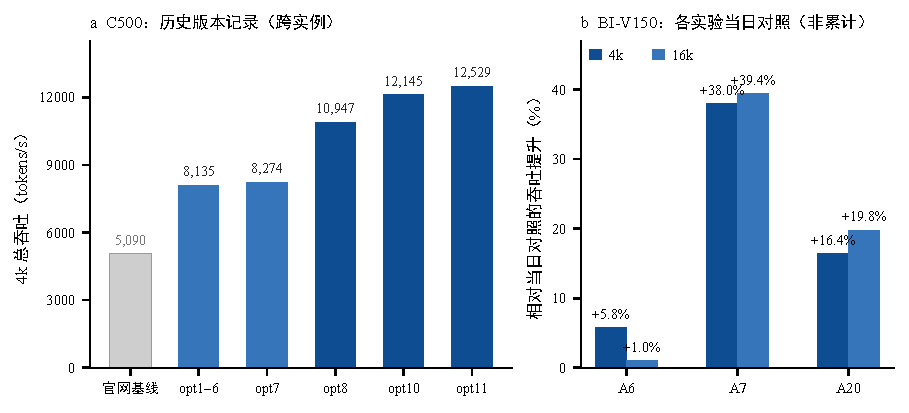
\includegraphics[width=\linewidth]{fig16_incremental_gains.pdf}
\caption{优化阶段的吞吐收益：C500 为跨实例历史版本记录，BI-V150 为各实验的当日对照\label{fig:incremental}}
\end{figure}

局部加速与端到端收益的关系见图~\ref{fig:speedup}。其中 opt8 的横坐标为四种 prefill GEMM 形状加速比的算术平均值，A20 为 stock 0.939 ms 与页对齐版本 0.588 ms 之比。由于各内核在完整模型中的时间占比不同，局部加速比与端到端提升之间不存在固定的线性换算关系。

\begin{figure}[!htbp]
\centering
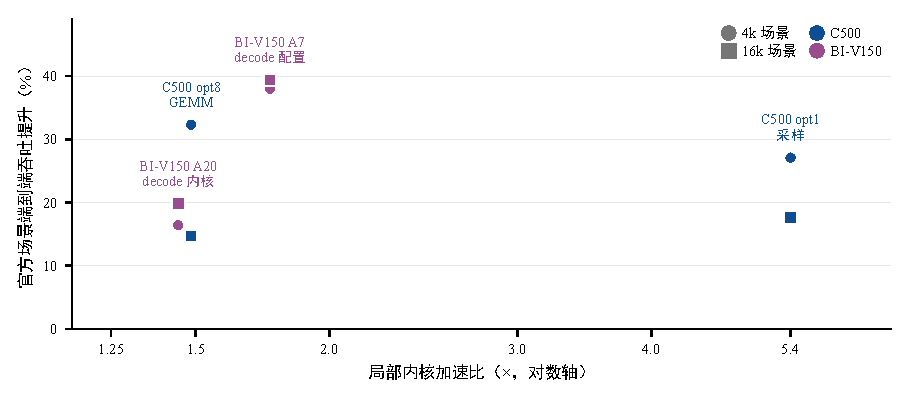
\includegraphics[width=\linewidth]{fig17_speedup_benefit.pdf}
\caption{局部内核加速比与官方场景端到端吞吐提升的关系\label{fig:speedup}}
\end{figure}

图~\ref{fig:efficiency} 进一步比较内核效率。左图将 decode attention 带宽分别归一到同芯片的实测参考：BI-V150 使用 copy 587 GB/s，C500 使用 sum 1610 GB/s；两种参考不作为跨芯片的绝对性能排名。右图给出 C500 四种 prefill GEMM 形状的计算吞吐，Triton 数值由相同矩阵运算量与实测耗时计算。

\begin{figure}[!htbp]
\centering
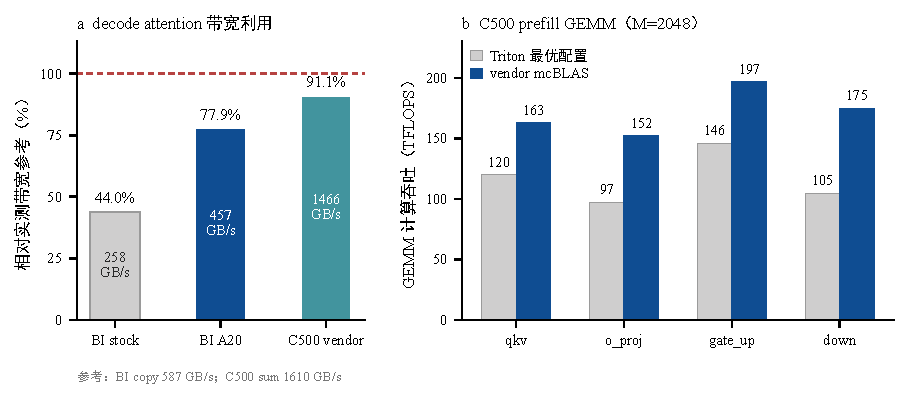
\includegraphics[width=\linewidth]{fig18_efficiency.pdf}
\caption{decode attention 带宽利用与 C500 prefill GEMM 计算吞吐\label{fig:efficiency}}
\end{figure}

\section{正确性验证}
正确性检查覆盖内核数值、批量不变性、采样分布和端到端精度。各层的测试对象、开发记录与当前状态见下表。

\begin{table}[!htbp]
\centering\small
\caption{正确性验证矩阵：从单个 kernel 到完整服务}
\begin{tabularx}{\linewidth}{@{}p{3.0cm}p{4.3cm}Y@{}}
\toprule
验证层 & 对象与方法 & 开发记录与状态 \\
\midrule
bit-exact & A6 双 gather、A7 发射配置 & A6 与两次 \texttt{index\_select} 逐位一致；A7 与 stock 的 \texttt{max\_diff}=0.0 \\
数值误差 & A20 vs stock，含 ragged 形状 & 等长最大 $3.05\times10^{-5}$，ragged 最大 $6.10\times10^{-5}$ \\
批量不变性 & 单条／两条／半批／全批／逆序全批，对照 fp32 & BI-V150 实测 9 passed \\
采样等价 & greedy、top-p、Gumbel 与 TV 距离 & greedy 与 \texttt{torch.argmax} 完全一致；保留集 IoU $\geq 0.999$；TV 与参考实现同档 \\
端到端精度 & evalscope MATH-500 Level 3（105 题） & C500 两次均为 98.1\%；BI-V150 为 96.19\% 和 98.1\% \\
真实路径命中 & 混合步 decode 切片 used/skipped & 当前日志 used=132000、skipped=0，未见 decode fast-path 异常回退 \\
启动验证 & 固定交付源码路径 + 独立 venv + 官方启动 & 当前 C500 交付版 293 秒启动，官方四轮 benchmark 与两次精度评测均完成 \\
\bottomrule
\end{tabularx}
\end{table}

\section{合规对照与复现指南}
\subsection{合规对照}
\begin{table}[!htbp]
\centering\small
\caption{赛题约束与本提交做法}
\begin{tabularx}{\linewidth}{@{}p{4.0cm}Y@{}}
\toprule
约束 & 本提交做法 \\
\midrule
\texttt{vllm serve} 参数与基线一致 & 两张卡均按官网原命令启动，未增删任何参数；C500 不额外添加 \texttt{--compilation-config}\\
禁止 benchmark 脚本调优 & 未修改官方脚本；当前 C500 与历史 opt 采用四轮去首后三轮均值，其他单次测量单独标明\\
禁止直接 merge 上游分支 & 基线为 flagos-2026-s2 与 FlagGems v5.3.5，全部改动以补丁形式叠加\\
算子优化须有开发量 & 新增 Triton 内核（paged decode attention、采样链、dual-gather）与路由/同步改造，均可独立 A/B\\
禁止改超参开启量化、投机采样 & 保持官方模型精度与生成配置，不启用量化或投机采样\\
精度 $\geq 0.95$ & C500 两次均为 98.1\%；BI-V150 为 96.19\% 和 98.1\%\\
TTFT 上限为官网 baseline +1\% & 两平台各场景均满足：BI 4k 为 4.14–4.33 s，低于官网 11.57 s；BI 16k 为 111.64–111.67 s，低于官网 599.26 s。同日 A/B 中 BI 4k 的 A20-1 相对 A7-1 为 +2.1\%，另一组为 −1.9\%；该对照用于分离 A20 收益，不替代官网基线判断\\
\bottomrule
\end{tabularx}
\end{table}

\subsection{复现步骤}
先取得两个集成分支（保留完整历史），再分别以可编辑模式安装：

\begin{reportcode}{源码获取与安装}
\begin{minted}{bash}
git clone --single-branch --branch integration/vllm-plugin-fl \
  https://github.com/xy200303/vllm-plugin-FL.git vllm-plugin-FL
git clone --single-branch --branch integration/flaggems \
  https://github.com/xy200303/FlagGems.git FlagGems

cd vllm-plugin-FL && pip install -e . --no-build-isolation
cd ../FlagGems   && pip install -e . --no-build-isolation
\end{minted}
\end{reportcode}

两平台均设置 \texttt{VLLM\_PLUGINS=fl}。C500 还需以下环境变量；当镜像已有其他版本的插件时，同时固定源码路径，避免加载到非交付目录：

\begin{reportcode}{C500 环境变量}
\begin{minted}{bash}
export PATH=/opt/conda/bin:$PATH
export MACA_PATH=/opt/maca
export MACA_HOME=/opt/maca
export LD_LIBRARY_PATH=/opt/maca/lib:/opt/maca/lib64
export VLLM_PLUGINS=fl
export PYTHONPATH=/workspace/vllm-plugin-FL:/workspace/FlagGems/src
\end{minted}
\end{reportcode}

启动命令与官网完全一致，天数在官方命令后追加编译配置，C500 不追加：

\begin{reportcode}{官方启动命令（与基线一致）}
\begin{minted}{bash}
# 天数 BI-V150
vllm serve /workspace/MiniCPM5-2B --port 9031 --served-model-name minicpm \
  --gpu-memory-utilization 0.85 --max-model-len 131072 \
  --compilation-config '{"cudagraph_mode": "FULL_DECODE_ONLY"}'

# 沐曦 C500（不添加 --compilation-config）
vllm serve /workspace/MiniCPM5-2B --port 9031 --served-model-name minicpm \
  --gpu-memory-utilization 0.85 --max-model-len 131072
\end{minted}
\end{reportcode}

性能评测执行官方脚本并传入两个官方用例：

\begin{reportcode}{官方性能评测命令}
\begin{minted}{bash}
python3 vllm-plugin-FL/benchmarks/benchmark_throughput_serve.py \
  --model /workspace/MiniCPM5-2B --served-model-name minicpm --port 9031 \
  --test-cases '[[4096,1024,64,256],[16384,1024,64,128]]'
\end{minted}
\end{reportcode}

精度评测执行官网给出的 evalscope 命令。结果位于工作目录的 \path{<timestamp>/reports/minicpm/math_500.json}；当前 evalscope 版本的精度字段为 \texttt{metrics[0].score}。

\subsection{复现注意事项}
（1）检查 prefix cache：benchmark 使用 seed=0，同一 serve 上重复相同 input\_len 的负载可能命中 prefix cache；本队日志出现过 35.9\% 命中率，并伴随 prefill 开销降低和吞吐虚高。旧日志不能证明各次运行均无命中，因此每个数据点都须检查命中率日志，必要时在新启动的 serve 上测量。当前交付复测的命中率低于 1\%。

（2）C500 需要 $\geq$128 GB CPU 内存：在模力方舟 64 GB 内存规格实例上，纯镜像原版 \texttt{vllm serve} 也会在 inductor 编译阶段被 cgroup OOM killer 杀掉（匿名内存峰值 63.4 GB，被杀时 GPU 显存仅 858 MiB，与显存、负载、代码改动均无关）。128 GB 规格实例全程稳定。

（3）启动耗时：C500 需执行 GEMM autotune 预热。当前交付复测启动为 293 秒，原生基线为 161 秒；预热时间随实例和缓存状态变化，不能用固定秒数估计。

（4）测量波动：C500 当前交付 4k 后三轮吞吐极差为 0.80\%，16k 为 0.29\%。BI-V150 两组 A20 的 4k 绝对值差异较大，因此两组均列出，不用单组高值代替整体结果；16k 两组基本一致。C500 同时保留官网与本机原生基线，避免跨实例参照混淆。

\section{结论}
本文在官方 FlagOS 栈上完成了 MiniCPM5-2B 的双平台推理优化。C500 的主要收益来自采样链融合、GEMM 路由和 prefill 同步消除；BI-V150 的主要收益来自 vendor attention 接入、发射配置调整和 paged decode attention 重写。当前交付的 C500 复测中，4k 与 16k 吞吐分别为官网基线的 2.44 倍和 1.57 倍，为本机原生基线的 2.95 倍和 1.88 倍。BI-V150 两组 A20 的 4k 为 4087.91 和 4722.22 tok/s，16k 为 4520.19 和 4520.10 tok/s；相对 A7 分别提升 6.0\%／22.9\% 和 26.7\%／26.6\%。C500 两次 MATH-500 均为 98.1\%，BI-V150 为 96.19\% 和 98.1\%。

当前交付复测的 C500 4k TTFT 为 1719.18 ms，16k TTFT 为 18141.47 ms，均优于官网和本机原生基线；BI-V150 的 16k TTFT 为 111.64–111.67 s，较 A7 降低约 18.5\%。后续可继续研究 prefill 分块策略和编译器融合，并在更多国产芯片上检验这些实现的适用性。

\begin{thebibliography}{9}
\bibitem{gb7713} 中华人民共和国国家质量监督检验检疫总局, 中国国家标准化管理委员会. GB/T 7713.3-2014 科技报告编写规则[S]. 北京: 中国标准出版社, 2014.
\bibitem{vllm} KWON W, LI Z, ZHUANG S, et al. Efficient memory management for large language model serving with PagedAttention[C]//Proceedings of the 29th ACM Symposium on Operating Systems Principles (SOSP). 2023: 611-626.
\bibitem{fa2} DAO T, FU D Y, ERMON S, et al. FlashAttention: fast and memory-efficient exact attention with IO-awareness[C]//Advances in Neural Information Processing Systems (NeurIPS). 2022.
\bibitem{gumbel} MADDISON C J, MNIH A, TEH Y W. The concrete distribution: a continuous relaxation of discrete random variables[C]//International Conference on Learning Representations (ICLR). 2017.
\bibitem{vfl} FlagOS Community. vllm-plugin-FL, branch flagos-2026-s2[EB/OL]. \url{https://github.com/flagos-ai/vllm-plugin-FL}.
\bibitem{fg} FlagOS Community. FlagGems, tag v5.3.5[EB/OL]. \url{https://github.com/flagos-ai/FlagGems}.
\bibitem{minicpm} OpenBMB. MiniCPM5-2B[EB/OL]. \url{https://modelscope.cn/models/OpenBMB/MiniCPM5-2B}.
\end{thebibliography}

\appendix
\section{代码与实验记录索引}
代码分支：插件为 \texttt{xy200303/vllm-plugin-FL} 的 \texttt{integration/vllm-plugin-fl}（C500 opt1–opt11、天数 A1–A7 与 A20，至 0207b7e1）；算子为 \texttt{xy200303/FlagGems} 的 \texttt{integration/flaggems}（采样融合内核、GEMM、paged\_decode\_attention 与测试，至 aff68555）。两者均为对应上游项目的正式 fork；历史开发线归档于 \texttt{archive/*}，官方基线保留于 \texttt{baseline/*}。报告与实验记录另存于 \texttt{xy200303/minicpm-flagserve} 的 \texttt{main}。

\begin{table}[!htbp]
\centering\small
\caption{关键代码文件与报告章节的对应关系}
\begin{tabularx}{\linewidth}{@{}p{6.1cm}Y@{}}
\toprule
文件（相对各自源码根目录） & 作用与对应章节 \\
\midrule
\path{vllm_fl/dispatch/backends/vendor/metax/patches/sampler_tail_fusion.py} & C500 采样链接入，§4.2 \\
\path{vllm_fl/dispatch/backends/vendor/metax/patches/linear_nn_repack.py} & nn 权重复本与形状路由，§4.3 \\
\path{vllm_fl/dispatch/backends/vendor/metax/patches/mcblas_mm.py} & ctypes 直调 vendor mcBLAS，§4.3 \\
\path{vllm_fl/dispatch/backends/vendor/metax/impl/attention/flash_attn.py} & prefill metadata 的当步 cumsum 缓存，§4.4 \\
\path{vllm_fl/dispatch/backends/vendor/iluvatar/impl/vendor_flash_attn.py} & vendor prefill、混合步拆分、双 gather，§5.2 \\
\path{vllm_fl/dispatch/backends/vendor/iluvatar/impl/decode_attn_pin.py} & 3D decode 发射配置，§5.3 \\
\path{vllm_fl/dispatch/backends/vendor/iluvatar/impl/decode_attn_fast.py} & A20 资格检查、slab、混合步回退，§5.4–5.5 \\
\path{src/flag_gems/fused/top_p_sample.py} & 直方图 top-p 与 Gumbel-Max，§4.2 \\
\path{src/flag_gems/fused/paged_decode_attention.py} & A20 分段内核与 combine，§5.4 \\
\path{tests/test_paged_decode_attention.py} & 精度与批量不变性测试，§5.5、§6 \\
\bottomrule
\end{tabularx}
\end{table}

实验记录：\path{docs/baselines/metax-c500/}（C500 基线与 opt1–opt11 逐项记录）、\path{docs/baselines/iluvatar-biv150/}（天数 A1–A9 记录）、\texttt{docs/experiments/}（后续实验、台账 \texttt{tracking.md} 与 \texttt{runs/} 原始数据）。目录中包含配置、serve 日志、benchmark CSV 和机器状态。

\subsection{结果与原始证据对应表}
以下路径均相对于文档仓库 \href{https://github.com/xy200303/minicpm-flagserve}{xy200303/minicpm-flagserve} 的根目录。汇总 CSV 可由同目录原始 CSV 复算，精度取 JSON 的 \texttt{metrics[0].score}；日志同时保留启动参数、实际加载路径和逐轮运行过程。

\begin{table}[!htbp]
\centering\small
\caption{报告结果、代码版本与原始证据索引}
\begin{tabularx}{\linewidth}{@{}p{2.5cm}p{4.2cm}Y@{}}
\toprule
结果 & 代码 / 对照 & 原始证据（路径与文件）\\
\midrule
C500 交付性能 & 插件 0207b7e1；算子 aff68555 & \path{docs/experiments/runs/c500-final-audit/healthy-final-raw.csv}；\texttt{healthy-final-summary.csv}；\texttt{healthy-final-serve.log} \\
C500 原生基线 & 插件 13eb9be；FlagGems v5.3.5 & 同目录 \texttt{healthy-baseline-raw.csv}、\texttt{healthy-baseline-summary.csv}、\texttt{healthy-baseline-serve.log} \\
C500 精度与微基准 & 当前交付提交 & 同目录 \texttt{healthy-eval1-math500.json}、\texttt{healthy-eval2-math500.json}、\texttt{micro-healthy.json}；环境见 \texttt{healthy-final-manifest.txt} \\
BI-V150 两组 A/B & A7 对照与 A20；同一交付提交内开关切换 & \path{docs/experiments/runs/bi-final-audit/1-a7/benchmark_results/}、\texttt{1-a20/}、\texttt{2-a7/}、\texttt{2-a20/} 下的 \texttt{benchmark\_results/}；同级 serve／bench 日志 \\
BI-V150 精度 & 当前交付提交 & 同目录 \texttt{eval1-math500.json}、\texttt{eval2-math500.json}、\texttt{eval-serve.log} \\
BI-V150 内核验证 & A20 与 stock & 同目录 \texttt{micro.json}、\texttt{pytest-a20.log}、\texttt{manifest.txt}；测试脚本为 \path{docs/verification/bi_micro_audit.py} \\
\bottomrule
\end{tabularx}
\end{table}

\subsection{官网基线来源}
官网基线位于赛题页面“4.3 评审方案”的“天数基线”和“沐曦基线”图片中，访问日期为 2026-10-27：\url{https://flagos.io/race-detail-season2?id=539vlt2p&lang=cn}。原图随报告源文件保存为 \texttt{official\_baseline\_biv150.png} 与 \texttt{official\_baseline\_c500.png}；图~\ref{fig:official-baselines} 原样展示，报告表 3 的官网基线数字由这两张表读取。

\begin{figure}[!htbp]
\centering
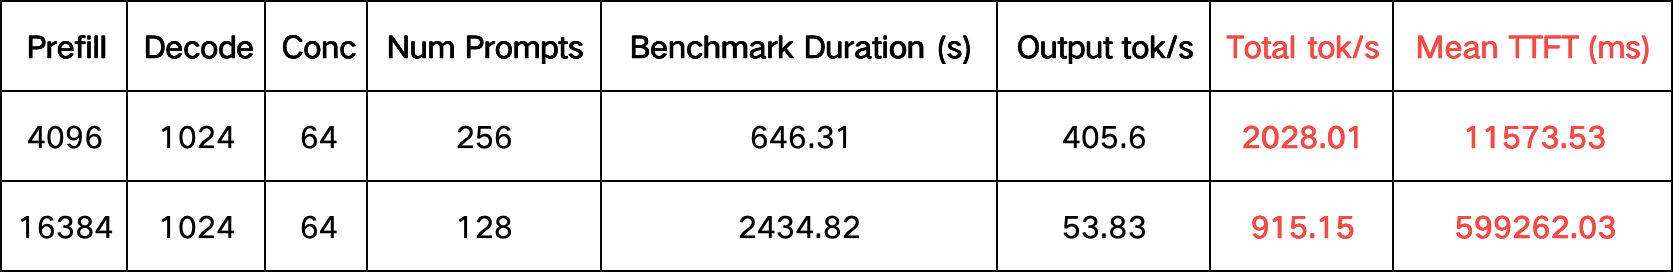
\includegraphics[width=\linewidth]{official_baseline_biv150.png}\\[5pt]
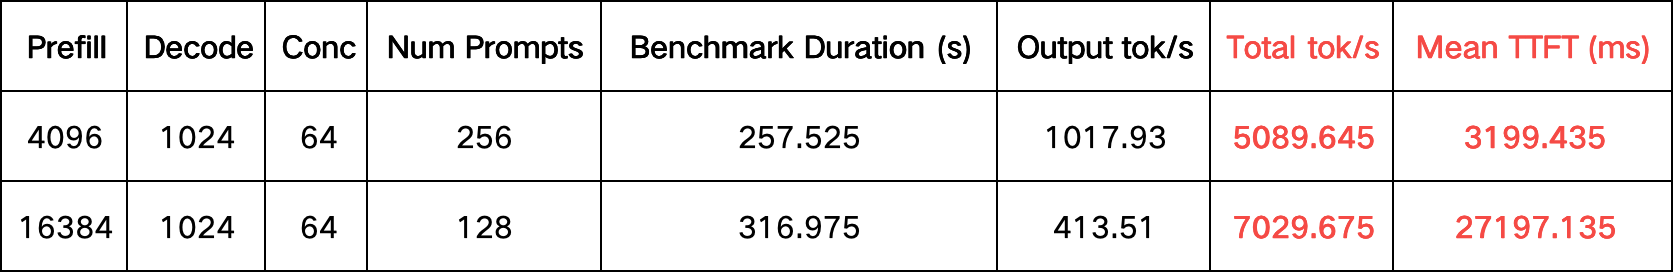
\includegraphics[width=\linewidth]{official_baseline_c500.png}
\caption{官网天数 BI-V150（上）与沐曦 C500（下）基线原图\label{fig:official-baselines}}
\end{figure}

原始图片地址分别为 \href{https://flagos.ks3-cn-beijing.ksyuncs.com/images/QlVfSLuI/image.png}{天数基线}和 \href{https://flagos.ks3-cn-beijing.ksyuncs.com/images/1a2hydOd/image.png}{沐曦基线}。官网基线用于统一赛题参照；本机原生基线和 A7 当日对照用于分析实际代码收益，三种参照在正文中分别标明，不相互替代。

\section{内核形状扫描与测量波动}
本附录给出 paged decode attention 在 NSEG $\times$ 并发度上的实测分布，以及官方 benchmark 连续 4 次 run 的吞吐波动。数据来源分别为 \texttt{docs/experiments/a26/a26\_sweep.log}（20 次重复取均值）和 \texttt{docs/baselines/metax-c500/raw\_runs\_baseline.csv}。

\begin{figure}[!htbp]
\centering
\begin{minipage}[b]{0.495\linewidth}
  \centering
  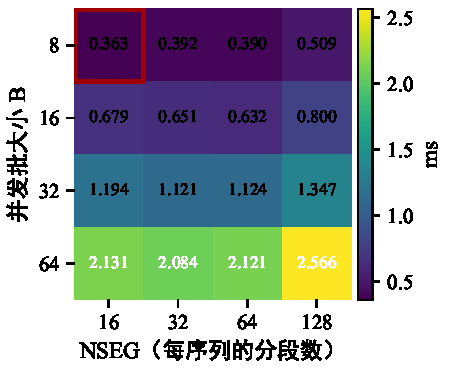
\includegraphics[width=\linewidth]{fig10_nseg_heatmap_16k.pdf}
  \subcaption{单层耗时（ms/层）}
\end{minipage}\hfill
\begin{minipage}[b]{0.495\linewidth}
  \centering
  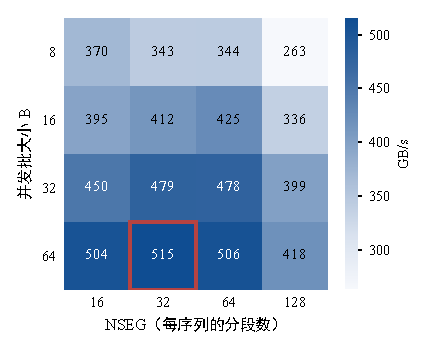
\includegraphics[width=\linewidth]{fig11_nseg_bw_16k.pdf}
  \subcaption{有效带宽（GB/s）}
\end{minipage}
\caption{NSEG $\times$ 并发度的实测分布（kv=16384）：红框为各自最优格}
\end{figure}

\begin{figure}[!htbp]
\centering
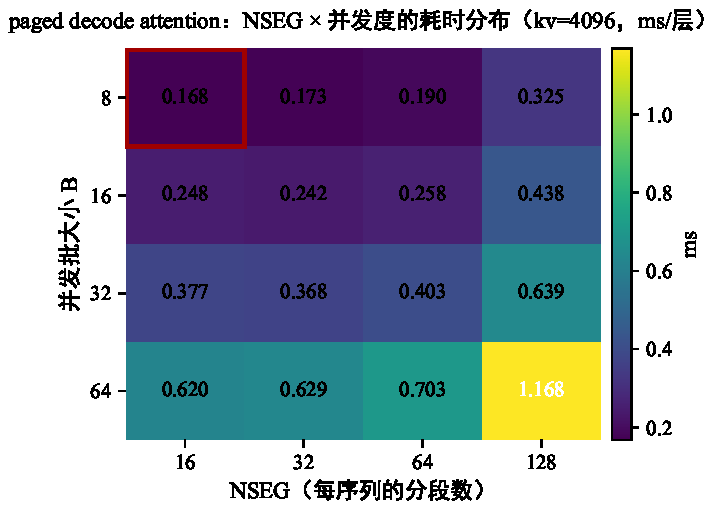
\includegraphics[width=\linewidth]{fig10b_nseg_heatmap_4k.pdf}
\caption{4k 场景下 NSEG $\times$ 并发度的单层耗时分布（kv=4096，ms/层）}
\end{figure}

官方 c64 形状下，NSEG=32 的有效带宽最高，为 515 GB/s，是实测 copy 参考 587 GB/s 的约 88\%；继续增大 NSEG 会增加归并开销。小 batch 调整 NSEG 可获得 3\%–7.4\% 的收益，但官方两个用例均为 c64，因此当前实现保留 NSEG=32。

\begin{figure}[!htbp]
\centering
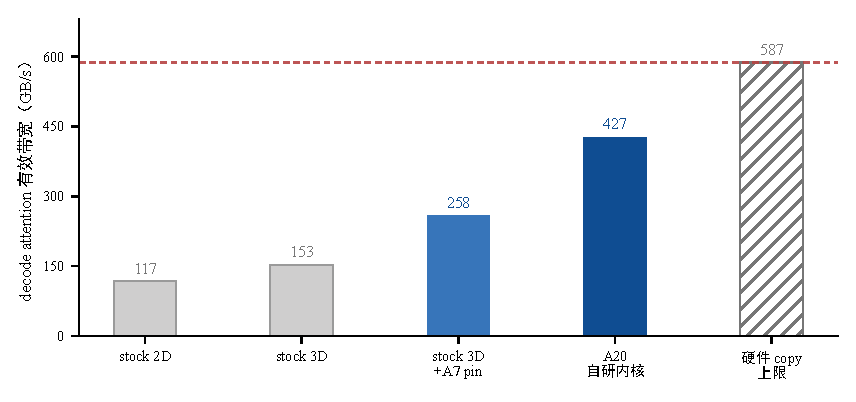
\includegraphics[width=\linewidth]{fig12_decode_evolution.pdf}
\caption{decode attention 从 stock 到自研内核的带宽演进}
\end{figure}

\begin{figure}[H]
\centering
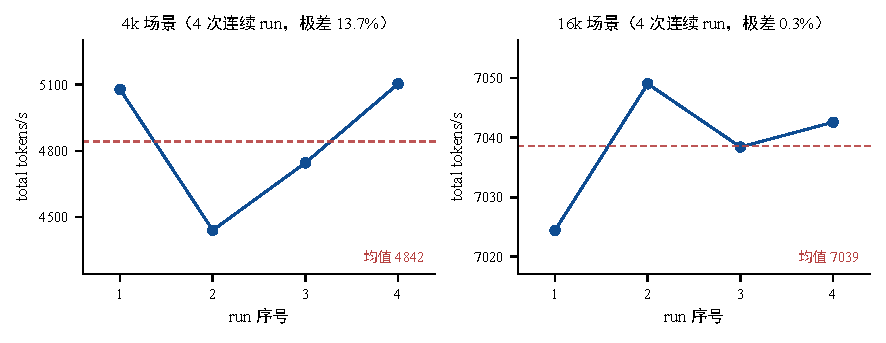
\includegraphics[width=\linewidth]{fig13_run_variance.pdf}
\caption{官方 benchmark 连续 4 次 run 的吞吐波动}
\end{figure}

官方 benchmark 对 4k 与 16k 均执行四轮，去掉首轮后取后三轮均值；历史 opt 系列采用这一口径。C500 区间端点及个别旧 16k 记录为单次 \texttt{vllm bench serve} 输出，已另行说明，不与四轮聚合混称。优化项使用同日交错 A/B 比较，减少实例时段漂移的影响。

\end{document}
